\documentclass[diss,capa]{texufpel}

\usepackage[utf8]{inputenc}
\usepackage{graphicx}
\usepackage[T1]{fontenc}

\hypersetup{
    hidelinks,
    unicode=true,
    linktoc=all
}

\unidade{Centro de Desenvolvimento Tecnológico}
\programa{Programa de Pós-Graduação em Computação}
\curso{Ciência da Computação}

\unidadeeng{Technology Development Center}
\programaeng{Postgraduate Program in Computing}
\cursoeng{Computer Science}

\title{Aplicação de Técnicas de Mineração de Dados e Learning Analytics para Predição de Evasão de Alunos na UFPel}

\author{Costa}{Alexandre Gomes da}
\advisor[Prof.~Dr.]{Mattos}{Julio Carlos Balzano de}
\coadvisor[Prof.~Dr.]{Primo}{Tiago Thompsen}
% \collaborator[Prof.~Dr.]{Aguiar}{Marilton Sanchotene de}

%Palavras-chave em PT_BR
\keyword{mineração de dados educacionais}
\keyword{learning analytics}
\keyword{técnicas de predição}
\keyword{kdd}
\keyword{descoberta de conhecimento em base de dados}

%Palavras-chave em EN_US
\keywordeng{educational data mining}
\keywordeng{learning analytics}
\keywordeng{prediction techniques}
\keywordeng{kdd}
\keywordeng{knowledge-discovery in databases}

\begin{document}

\maketitle 

\sloppy

\fichacatalografica

%Composição da Banca Examinadora
\begin{aprovacao}{01 de agosto de 2020} %data da banca por extenso
\noindent Prof. Dr. Julio Carlos Balzano de Mattos (orientador)\\
Doutor em Computação pela Universidade Federal do Rio Grande do Sul.\\[1cm]

\noindent Prof. Dr. Tiago Thompsen Primo\\
Doutor em Computação pela Universidade Federal do Rio Grande do Sul.\\[1cm]

\noindent Prof. Dr. Ricardo Matsumura Araujo\\
Doutor em Computação pela Universidade Federal do Rio Grande do Sul.\\[1cm]

\noindent Prof. Dr. Luciano da Silva Pinto\\
Doutor em Biotecnologia pela Universidade Federal de Pelotas.
\end{aprovacao}

%Opcional
\begin{dedicatoria}
  Dedico\ldots 
\end{dedicatoria}

%Opcional
\begin{agradecimentos}
  Agradeço\ldots 
\end{agradecimentos}

%Opcional
\begin{epigrafe}
  Tudo o que não puder contar como fez; Não o faça! Se há razões para não contar; há para não o fazer.\\
  {\sc --- Kant}
\end{epigrafe}

%Resumo em Portugues (no maximo 500 palavras)
\begin{abstract}
Os sistemas de gestão para educação armazenam uma grande quantidade de dados oriundos de diversas modalidades de iteração entre alunos e professores mas também entre os alunos e o ambiente educacional (biblioteca, restaurantes universitários entre outros). Por exemplo, dados como notas, registro de presença de aluno, acesso ao sistema de biblioteca, logs de iteração com o sistema e vários outros tipos de atributos são ricos para a compreensão e auxílio nos processos de tomada de decisão em ambientes educacionais. Analisar e encontrar padrões nesta quantidade de dados manualmente é inviável humana e economicamente, por isso a utilização de Mineração de Dados Educacionais (MDE) e \textit{Learning Analytics (LA)} ganharam popularidade nos últimos anos. Este trabalho pretende explorar a utilização destas técnicas para extrair os dados do Sistema Integrado de Gestão da UFPel (Cobalto) visando criar modelos que levem a predição de alunos em risco de evasão para suporte aos processos de tomada de decisão na Universidade Federal de Pelotas.
\end{abstract}

%Resumo em Inglês (no maximo 500 palavras)
\begin{englishabstract}{Application of Data Mining Techniques and Learning Analytics for Student Dropout Prediction at UFPel}
Management systems for education store a large amount of data from various classes of interaction between students and teachers, but also between students and the educational environment (library, university restaurants and others). For example, data such as grades, student attendance records, library system access, system iteration logs, and various other types of attributes are rich for understanding and aiding decision-making processes in educational settings. Analyzing and finding patterns in this amount of data manually is not feasible and economically human, so use Educational Data Mining (MDE) and Learning Analytics (LA) to gain popularity in recent years. This paper aims to explore the use of these techniques to extract data from the UFPel (Cobalto) Integrated Management System, using modeling models that predict students at risk of dropping out to support decision-making processes at the Federal University. from Pellets.
\end{englishabstract}

%Lista de Figuras
\listoffigures

%Lista de Tabelas
\listoftables

%lista de abreviaturas e siglas
\begin{listofabbrv}{ABNT}%coloque aqui a maior sigla para ajustar a distância
        \item[ABNT] Associação Brasileira de Normas Técnicas
        \item[NUMA] Non-Uniform Memory Access
        \item[SIMD] Single Instruction Multiple Data
        \item[SMP] Symmetric Multi-Processor
        \item[SPMD] Single Program Multiple Data
\end{listofabbrv}

%Sumario
\tableofcontents

\chapter{Introdução}

O uso constante de Tecnologia da Informação e Comunicação em diversas áreas vêm gerando um grande volume de dados. Tecnologias como a internet, redes sociais, ambientes virtuais de aprendizagem, dispositivo móveis, aplicativos embarcados, leitores de código de barras, sensores, leitores biométricos e sistemas de informação em geral são alguns exemplos de recursos que vem aumentando o número de dados das mais diversas naturezas \cite{goldschmidt2015data}.

%% Educação
Atualmente, as áreas como a educação produzem uma grande quantidade de dados relacionados a alunos e professores todos os dias. Para isto, esta área utiliza sistemas para fazer o controle de iterações acadêmicas, gestão de projetos de pesquisa, ensino ou extensão, ou até mesmo sistemas para fazer o controle de gestão de pessoas são alguns do exemplos de sistemas que podem gerar um volume considerável de dados com frequência.

A partir desse volume de dados é possível analisar problemas recorrentes relacionados a educação. Um desses problemas é a evasão escolar que ainda é um desafio a ser superado.
A evasão é um problema que atinge não só as Instituições de Ensino Superior (IES) privadas, mas também as públicas. Segundo dados do \citet{inep:2018}, em 2017, o índice de matrículas desvinculadas em todo o Brasil foi de 16,41\%. Já para as IES públicas esse índice no mesmo período foi de 11,56\%. Outro valor a ser considerado é o número de matriculas trancadas, onde foi de 11,17\% em todo o Brasil e 8,10\% IES públicas.

Comparando os índices da Universidade Federal de Pelotas (UFPel) com os do \citet{inep:2018} estes índices não mudam muito. Em 2017 o índice de matriculas desvinculadas na UFPel foi de de 11,53\% que está abaixo do índice de 11,56\% apresentado pelo \citet{inep:2018}. Mas olhando para a evasão curso a curso no ano de 2017 observamos dados alarmantes. Por exemplo, temos cursos como o de Geoprocessamento onde a taxa de evasão foi de 29,07\%.  Esse fenômeno é conhecido na estatística como paradoxo de Simpson, uma tendência aparece em um determinado grupo de dados e desaparece quando estes dados são combinado. Ou seja, olhando para os cursos individualmente vários deles apresentam uma taxa de evasão bem elevada, mas quando essas taxas são combinadas a taxa de evasão não é tão relevante \cite{wagner1982simpson}. Olhando para esses dados algumas perguntas surgem tais como "Qual é o perfil do aluno que tende a evadir?" ou "Qual é a quantidade de alunos que trancaram e acabaram evadindo?", por exempo.

%% Knowledge Discovery in Database - KDD
Embora com ajuda de ferramentas computacionais, analisar essa crescente quantidade de dados não é trabalho para o homem \cite{goldschmidt2015data}. Para ajudar nesta questão a área de Descoberta de Conhecimento em Base de Dados (\textit{Knowledge Discovery in Database} - KDD) é focada em extrair conhecimento encima de granes volumes de dados. O termo mais conhecido relacionado a essa área é a Mineração de Dados (MD) que é uma das etapas do processo de KDD.

%% Mineração de dados educacionais
Segundo \citet{Koedinger2008} Mineração de Dados (MD) aplicada à educação é um campo interdisciplinar emergente mais conhecido como Mineração de Dados Educacionais (MDE).
\citet{baker2010data} define MDE como a área de investigação científica centrada no desenvolvimento de métodos para fazer descobertas dentro dos tipos de dados que vêm de ambientes educacionais e usando esses métodos para entender melhor os alunos e a aprendizagem deles. A Figura \ref{fig:areas-relacionadas-mde} mostra que a área de MDE pode ser a combinação de 3 grandes áreas (ciência da computação, estatistia e educação) e serve de exemplo para justificar a interdisciplinaridade da área.

\begin{figure}[htbp]
  \centering 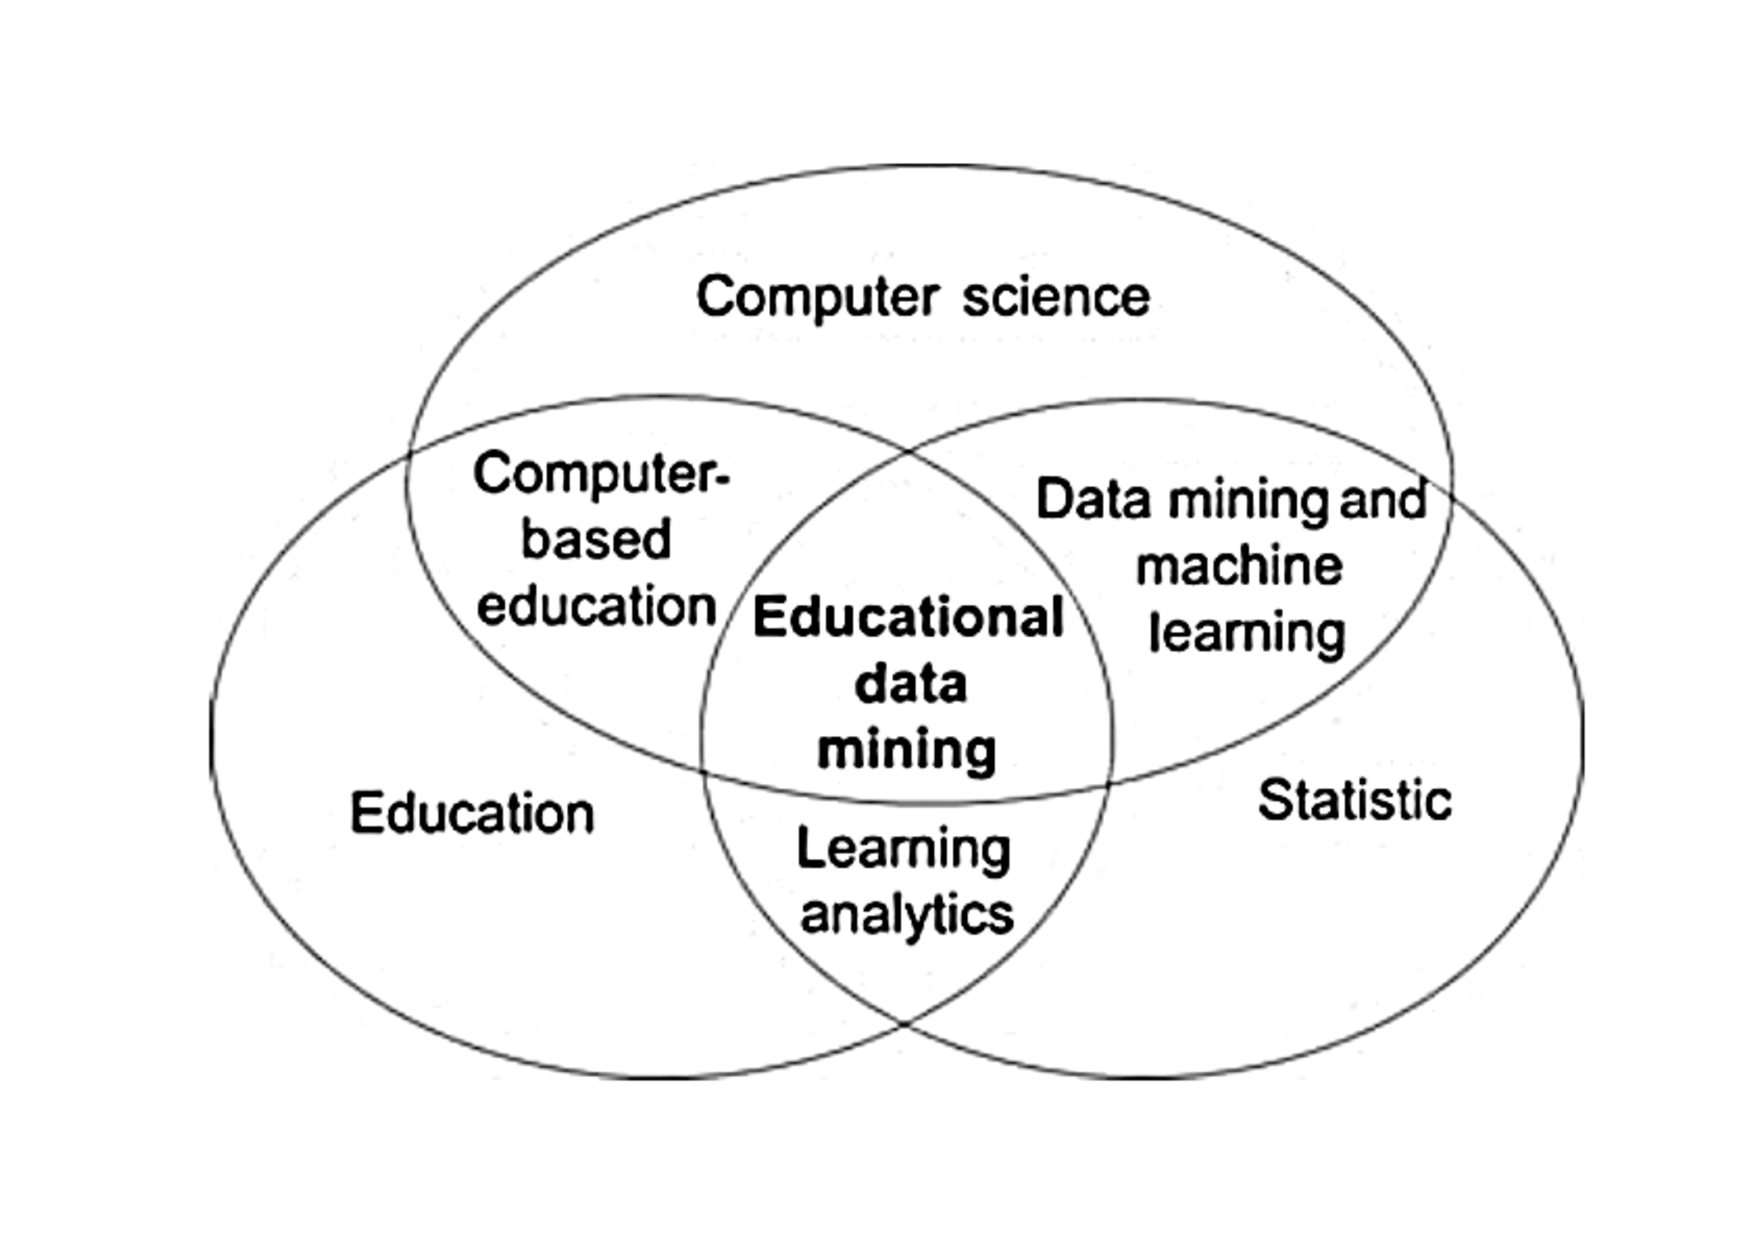
\includegraphics[scale=.4]{imagens/areas-edm.pdf}
  \caption{Principais áreas relacionadas com mineração de dados educacionais. \cite{Koedinger2008}}
  \label{fig:areas-relacionadas-mde}
\end{figure}

Neste trabalho iremos explorar a utilização de MDE/LA visando classificar e identificar perfis de alunos com tendência a evadir. Segundo \citet{goldschmidt2015data} uma tarefa de classificação possui dois grupos. Um grupo contem normalmente um atributo apenas que vai servir para fazer a predição de um valor (atributo-alvo). Outro grupo corresponde aos atributos que vão servir para fazer a predição do valor (atributos de predição). Tarefas de classificação são largamente utilizadas para fazer a predição de alunos em risco de evasão escolar, como será apresentado nesta proposta.

\citet{baker2010data} agrupa o problema de evasão em uma categoria ou tarefa de detectar o comportamento do aluno. Onde o objetivo é detectar os alunos que têm algum tipo de problema ou comportamento incomum, por exemplo: pouca motivação, trapaça, evasão escolar, etc. Destaca também que as principais técnicas usadas para resolver esses tipos de problemas são de classificação e agrupamentos.

%% 2014
No trabalho de \citet{rigo2014aplicaccoes} é apresentado um estudo de fatores envolvidos no fenômeno de evasão escolar e descrevem a utilização de um sistema para MDE e LA durante 18 meses em cursos de graduação na modalidade de Educação a Distância. Ao todo foram executados 4 experimentos onde foram acompanhados 603, 250, 925 e 713 alunos. Para cada estudo de caso que trata o trabalho foi utilizado a técnica \textit{RNA Multilayer Perceptron}. O melhor resultado com relação a predição da evasão foi no experimento 4 onde a melhor média de acertos foi de 83,7\%.

%% 2015
\citet{pradeep2015students} buscaram prever a evasão de alunos em \textit{middle or secondary education} de uma escola de renome na Índia. O conjunto de dados foi composto por 670 registros de alunos com 57 atributos de estudantes registrados entre 2011 e 2013. Foram usadas 3 fontes de dados diferentes pesquisa com familiares, formulários de admissão e notas dos alunos. O estudo utilizou a ferramenta WEKA: para a seleção de atributos utilizou 7 algoritmos (CfsSubsetEval, ReliefFAttributeEval, ChiSquaredAttributeEval, neRAttributeEval, Consistency-SubsetEval, Filtered AttributeEval, GainRatioAttributeEval) e para a classificação aplicou a técnica de \textit{Decision tree} e \textit{rule induction}. Segundo o autor a qualidade e a confiabilidade das informações disponíveis afetam diretamente os resultados obtidos, por isso é importante reunir as informações corretas. As principais considerações a respeito das técnicas de mineração de dados foram de que os algoritmos se mostraram promissores para fazer a predição de evasão, e a seleção de atributos contribuem para diminuir o número de regras e condições sem perder o desempenho dos classificadores. Com relação ao conhecimento extraído as principais conclusões foram: os métodos de \textit{decision tree} e \textit{induciton rule} são facilmente convertidos em regras \textit{IF-THEM}; alguns atributos que contribuem diretamente para a evasão são notas baixa em matemática, inglês e física, e também alunos com idade acima de 15 anos.

%% 2016
Em \citet{hasbun2016extracurricular} foi discutida a importância de atividades extracurriculares para prever o abandono escolar de estudantes de dois cursos de Bacharel em Ciências (Engenharia e Negócios). Foram coletados dados de 4840 alunos. Dois modelos foram treinados, uma incluindo todos os dados e outra removendo notas e créditos obrigatórios do valor das atividades. Ambos os modelos foram treinados e validados usando \textit{cross-validation}. Utilizou o pacote \textit{R Studio} para o algoritmo CART. A primeira árvore de decisão obteve a melhor precisão (93,94\%). Para o segundo modelo obteve uma precisão de 79,29\%. Os autores relataram que embora a previsão de abandono com dados acumulados mostre um melhor desempenho, o segundo modelo ajuda a resolver o problema de disponibilidade de dados dos alunos. Além disso, a partir da análise dos erros, descobriram que a árvore de decisão treinada com todos os dados foi eficiente na modelagem das expectativas acadêmicas do programa, ocultando fatores pessoais que são mais relevantes para intervenções de prevenção de abandono. Por isso, os resultados apresentados sugerem que incluir atividades extracurriculares é útil para observar comportamentos específicos que parecem estar relacionados ao fenômeno de desligamento relacionado ao abandono.

%% 2017

%% 2018
\citet{lanes2018prediccao} apresentaram um estudo que visa identificar estudantes que apresentam risco de evasão a partir do seu primeiro ano no curso de graduação. Os experimentos foram realizados com informações extraídas do sistema acadêmico da FURG. O conjunto de dados contou com 916 registros de 12 cursos de graduação de áreas distintas. Os dados foram discretizados e categorizados para gerar o \textit{dataset} final. Foi utilizado a ferramenta Weka e aplicado o algoritmo J48 para processar o \textit{dataset} e obter a arvore de decisão. Os resultados mostram que os potenciais alunos em risco de evadir podem ser identificados com acurácia de 90,7\% usando o algoritmo J48.

%% Justificativa

Este trabalho possui como motivação o grande problema de evasão encontrado nos cursos superiores, em especial em alguns cursos sendo principalmente cursos das engenharias e exatas, e a dificuldade de traçar o perfil destes alunos. Além disso, existe uma enorme quantidade de dados históricos de cursos de graduação presencias da UFPEL, uma vez que a grande maioria dos trabalhos vem de cursos EAD. Quanto alguns trabalhos fazem questionários, provas, exercícios, etc, no presente trabalho serão coletado dados que foram gerados a partir de resultado que os alunos obtiveram em diversas disciplinas, cursos entre outros. Este trabalho utilizará a base de dados do Sistema Integrado de Gestão da UFPEL (Cobalto). A base do Cobalto conta também com os dados históricos do GOL que foi o sistema acadêmico da UFPEL de 2006 à 2013.

\chapter{Referencial Teórico}

  Bla blabla blablabla bla.  Bla blabla blablabla bla.  Bla blabla
  blablabla bla.  Bla blabla blablabla bla.  Bla blabla blablabla bla.
  Bla blabla blablabla bla.  Bla blabla blablabla bla.  Bla blabla
  blablabla bla.  Bla blabla blablabla bla.  Bla blabla blablabla bla.
  Bla blabla blablabla bla.  Bla blabla blablabla bla.  Bla blabla
  blablabla bla.  Bla blabla blablabla bla.  Bla blabla blablabla bla.
  Bla blabla blablabla bla.  Bla blabla blablabla bla.  Bla blabla
  blablabla bla.  Bla blabla blablabla bla.  Bla blabla blablabla bla.
  Bla blabla blablabla bla.

\section{Evasão Escolar}

  Bla blabla blablabla bla.  Bla blabla blablabla bla.  Bla blabla
  blablabla bla.  Bla blabla blablabla bla.  Bla blabla blablabla bla.
  Bla blabla blablabla bla.  Bla blabla blablabla bla.  Bla blabla
  blablabla bla.  Bla blabla blablabla bla.  Bla blabla blablabla bla.
  Bla blabla blablabla bla.  Bla blabla blablabla bla.  Bla blabla
  blablabla bla.  Bla blabla blablabla bla.  Bla blabla blablabla bla.
  Bla blabla blablabla bla.  Bla blabla blablabla bla.  Bla blabla
  blablabla bla.  Bla blabla blablabla bla.  Bla blabla blablabla bla.
  Bla blabla blablabla bla.


\chapter{Trabalhos Relacionados}

  Bla blabla blablabla bla.  Bla blabla blablabla bla.  Bla blabla
  blablabla bla.  Bla blabla blablabla bla.  Bla blabla blablabla bla.
  Bla blabla blablabla bla.  Bla blabla blablabla bla.  Bla blabla
  blablabla bla.  Bla blabla blablabla bla.  Bla blabla blablabla bla.
  Bla blabla blablabla bla.  Bla blabla blablabla bla.  Bla blabla
  blablabla bla.  Bla blabla blablabla bla.  Bla blabla blablabla bla.
  Bla blabla blablabla bla.  Bla blabla blablabla bla.  Bla blabla
  blablabla bla.  Bla blabla blablabla bla.  Bla blabla blablabla bla.
  Bla blabla blablabla bla.

\chapter{Metodologia}

Neste trabalho será utilizado uma metodologia apresentada no livro de \citet{goldschmidt2015data}, que é baseada na metodologia CRISP-DM (Cross-Industry Standard Process for Data Mining) e em alguns princípios de planejamento de atividades. A metodologia mostrada no livro se difere da metodologia CRISP-DM no momento em que ela sugere aplicar a definição dos objetivos e escolha da técnica de mineração antes da faze de preparação dos dados. Além disso, ela adiciona instrumentos para documentar as decisões e os resultados durante o processo de KDD, um exemplo é o formulário mostrado na figura \ref{fig:formulario-para-documentacao-de-acoes}.

\begin{figure}[htbp]
  \centering 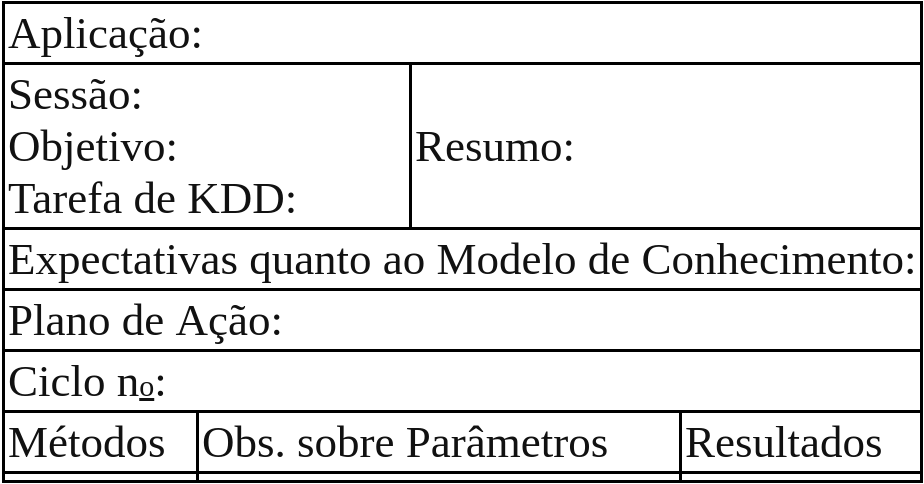
\includegraphics[scale=.4]{imagens/formulario-para-documentacao-de-acoes.png}
  \caption{Formulário para documentação de ações \cite{goldschmidt2015data}.}
  \label{fig:formulario-para-documentacao-de-acoes}
\end{figure}

A metodologia proposta no livo divide o processo em 5 etapas Levantamento da Situação Vigente, Definição dos Objetivos, Planejamento de Atividades, Execução dos Planos de Ação e Avaliação de Resultados. O resto desta sessão aprofunda cada uma dessas etapas.

\section{Levantamento da Situação Vigente}
\label{sec:levantamento-da-situacao-vigente}

Nesta etapa deve ser realizada todas as fases da \textbf{Compreensão do Negócio} e \textbf{Compreensão dos Dados} da metodologia CRISP-DM. 

A fase de \textbf{Compreensão do Negócio} tem como meta compreender o contexto em que o processo de KDD será realizado. As principais considerações técnicas desta fase são:
\begin{itemize}
\item Fazer a identificação das pessoas envolvidas no processo;
\item Elaborar uma lista de necessidades e expectativas das pessoas envolvidas quanto ao propósito do KDD;
\item Conhecer o software e hardware existentes;
\item Elaborar um inventário da base de dados;
\item Verificar se existe um Data Warehouse;
\item Tentar identificar e documentar todo o conhecimento prévio existente e disponível sobre o domínio da aplicação.
\end{itemize}

Na fase de \textbf{Compreensão dos dados} será feito um estudo detalhado das informações disponíveis. Esta fase vão ser realizadas as etapas destacadas abaixo:
\begin{itemize}
\item Compreender como um todo os dados e atributos disponíveis da base de dados;
\item Avaliar a qualidade dos dados disponíveis;
\item Verificar a disponibilidade dos dados, principalmente sobre a quantidade dos dados;
\end{itemize}

Já na etapa de levantamento vai ser usado o formulário da figura \ref{fig:formulario-para-documentacao-de-acoes} para documentação de ações e resultados do processo de KDD. O formulário deve ser utilizado para registrar o titulo da aplicação e um resumo descritivo do trabalho.


% É nesta etapa que será realizado um estudo mais aprofundado para tentar entender mais a fundo o problema da evasão e também tentar definir o objetivo sob a luz de descoberta de conhecimento em base de dados.

\section{Definição dos Objetivos}
\label{sec:definicao-dos-objetivos}

Na metodologia proposta do livro a etapa de Definição dos Objetivos agrega duas fazes da metodologia CRISP-DM Compreensão do Negócio e Modelagem. Essa etapa destaca que a escolha da técnica mineração deve vir antes da preparação dos dados, logo o pré-processamento dos dados pode seguir em função da técnica de mineração aplicada aos dados.

De forma prática primeiramente serão identificadas todas as expectativas, logo depois elas serão validadas junto aos Orientadores. Por fim, essas expectativas serão agrupadas de acordo com sua natureza e de forma que um modelo de conhecimento possa englobar um grupo de expectativas.

Com as expectativas identificas e agrupadas será apurado qual tipo de tarefa de Mineração de Dados deve ser aplicado para obter um modelo de conhecimento que atenda a cada grupo de expectativa.

Nesta etapa serão preenchidos os seguintes campos do formulário gerado na etapa anterior: Sessão, Objetivo, Tarefa de KDD e Expectativas quanto ao modelo de conhecimento.
Uma sessão estará associada a uma única tarefa de KDD. O objetivo será associado a um grupo de expectativas. A tarefa de KDD será a tarefa que será executada para o objetivo dessa sessão. Para o ultimo campo será especificado uma lista de expectativas quanto ao modelo de conhecimento.

A figura~\ref{fig:formulario-etapa-definicao-objetivo} é um exemplo de como preencher o formulário da sessão \ref{sec:levantamento-da-situacao-vigente}. É o exemplo da expectativa de comportamento do cliente que é mapeada em uma tarefa de Descoberta de Sequência.

\begin{figure}[htbp]
  \centering 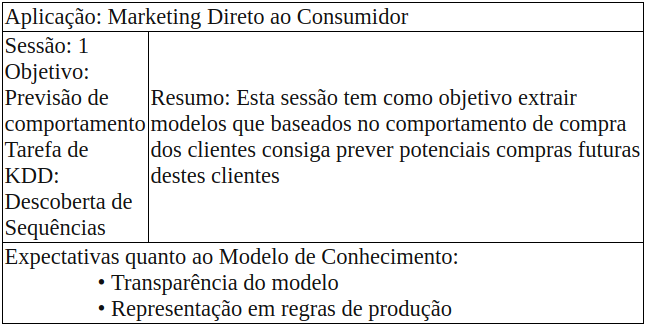
\includegraphics[scale=.4]{imagens/formulario-etapa-definicao-objetivo.png}
  \caption{Exemplo de preenchimento do formulário na etapa de Definição de Objetivos. Fonte: \cite{goldschmidt2015data}.}
  \label{fig:formulario-etapa-definicao-objetivo}
\end{figure}

\section{Planejamento de atividades}
\label{sec:planejamento-de-atividades}

Nesta etapa cada sessão de KDD identificada na sessão \ref{sec:definicao-dos-objetivos} deverá ser elaborado um planejamento de atividades que proporcione a execução do objetivo correspondente. Também será identificado, dentre o métodos disponíveis, aqueles que melhor implementam a tarefa da sessão de KDD. Este métodos são chamados de métodos candidatos.

Segundo \citet{goldschmidt2015data} a filtragem dos métodos requer conhecimento profundo de cada método e que a escolha do método depende da preferência pessoal do analista de KDD, porem ressalva que todos os métodos candidatos que não foram retirados da filtragem devem ser considerados. A filtragem dos métodos candidatos será feita junto aos orientadores e ao fim dessa filtragem será elaborado uma lista ordenada dos método que podem obter melhor resultado.

A partir da listagem dos métodos selecionados será apresentado alternativas de pré-processamento para cada método da lista. \citet{goldschmidt2015data} denomina essas alternativas de pré-processamento de planos de ação e que o analista deve planejar quais métodos de pré-processamento devem ser utilizados, incluindo a ordem de aplicação.

A figura \ref{fig:formulario-etapa-planejamento-atividades} é um exemplo retirado do livro que mostra como ficaria o formuláro após a etapa de planejamento de atividades.

\begin{figure}[htbp]
  \centering 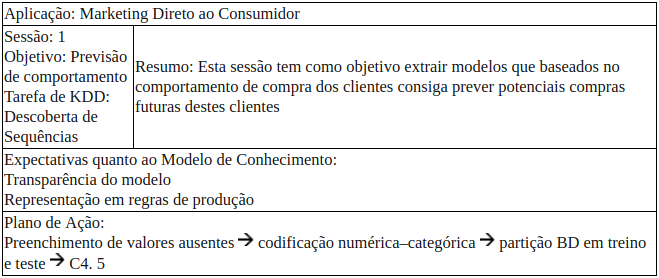
\includegraphics[scale=.4]{imagens/formulario-etapa-planejamento-atividades.png}
  \caption{Exemplo de preenchimento do formulário na etapa de Planejamento de Atividades. Fonte: \cite{goldschmidt2015data}.}
  \label{fig:formulario-etapa-planejamento-atividades}
\end{figure}

\section{Execução do Plano de Ação}
\label{sec:execucao-do-plano-de-acao}

Nesta etapa todos os planos de ação descritos na sessão \ref{sec:planejamento-de-atividades} serão experimentados e avaliados. \citet{goldschmidt2015data} recomenda que os planos sejam executados simultaneamente para ser feito uma análise conjunta dos resultados obtidos. Isso pode trazer uma visão global do processo e pode ser possível perceber detalhes que permitam reavaliar ou mudar a estratégia escolhida.

\citet{goldschmidt2015data} recomenda também que o plano de ação entende a execução ordenada dos métodos do plano e deve ser executada em ciclos. Ou seja, o plano deve ser executado total ou parcialmente a cada ciclo, procurando obter os melhores resultados.

\citet{goldschmidt2015data} destaca que um problema frequente em um processo de KDD é a escolha dos parâmetros de um algoritmo frente a uma nova situação. Este problema pode aumentar bastante o número de ciclos do processo. Por isso, nessa etapa serão registrados dos parâmetros adotados e os resultados obtidos a cada ciclo no formulário. A figura \ref{fig:formulario-etapa-execucao-dos-planos-de-acao} mostra um possível preenchimento do formulário.

\section{Avaliação de Resultados}
\label{sec:avaliacao-de-resultados}

Esta etapa deve ser realizada no final do processamento de cada método do plano. \citet{goldschmidt2015data} diz que é o momento de comparar as características do modelo de conhecimento gerado com as expectativas quanto ao modelo de conhecimento listadas na sessão \ref{sec:definicao-dos-objetivos}. Ele reforça que algumas medidas podem ser comparadas diretamente, já outras, são mais subjetivas. Uma pergunta que poderia se fazer nessa etapa é qual é a exclusividade e utilidade do conhecimento extraído? Por isso, esta etapa deverá ser homologada junto ao orientador deste trabalho. Nessa etapa também terá de ser feito um estudo sobre as medidas de interesse no processo de KDD.

\begin{figure}[htbp]
  \centering 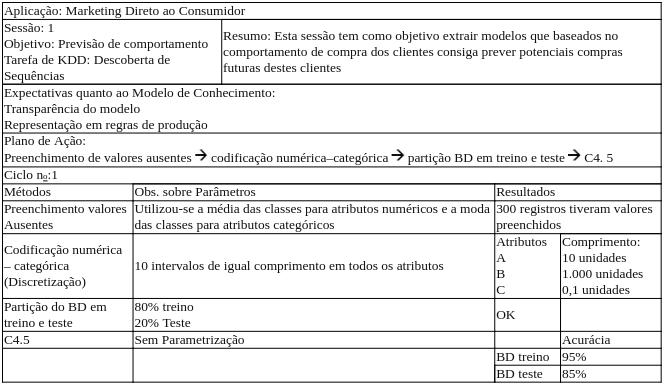
\includegraphics[scale=.4]{imagens/formulario-etapa-execucao-dos-planos-de-acao.png}
  \caption{Exemplo de preenchimento do formulário na etapa de Execução do plano de ação. Fonte: \cite{goldschmidt2015data}.}
  \label{fig:formulario-etapa-execucao-dos-planos-de-acao}
\end{figure}

\chapter{Experimentos}

  Bla blabla blablabla bla.  Bla blabla blablabla bla.  Bla blabla
  blablabla bla.  Bla blabla blablabla bla.  Bla blabla blablabla bla.
  Bla blabla blablabla bla.  Bla blabla blablabla bla.  Bla blabla
  blablabla bla.  Bla blabla blablabla bla.  Bla blabla blablabla bla.
  Bla blabla blablabla bla.  Bla blabla blablabla bla.  Bla blabla
  blablabla bla.  Bla blabla blablabla bla.  Bla blabla blablabla bla.
  Bla blabla blablabla bla.  Bla blabla blablabla bla.  Bla blabla
  blablabla bla.  Bla blabla blablabla bla.  Bla blabla blablabla bla.
  Bla blabla blablabla bla.

\chapter{Discussão dos Resultados}

  Bla blabla blablabla bla.  Bla blabla blablabla bla.  Bla blabla
  blablabla bla.  Bla blabla blablabla bla.  Bla blabla blablabla bla.
  Bla blabla blablabla bla.  Bla blabla blablabla bla.  Bla blabla
  blablabla bla.  Bla blabla blablabla bla.  Bla blabla blablabla bla.
  Bla blabla blablabla bla.  Bla blabla blablabla bla.  Bla blabla
  blablabla bla.  Bla blabla blablabla bla.  Bla blabla blablabla bla.
  Bla blabla blablabla bla.  Bla blabla blablabla bla.  Bla blabla
  blablabla bla.  Bla blabla blablabla bla.  Bla blabla blablabla bla.
  Bla blabla blablabla bla.

\chapter{Considerações Finais}

Bla blabla blablabla bla.  Bla blabla blablabla bla.  Bla blabla
blablabla bla.  Bla blabla blablabla bla.  Bla blabla blablabla bla.
Bla blabla blablabla bla.  Bla blabla blablabla bla.  Bla blabla
blablabla bla.  Bla blabla blablabla bla.  Bla blabla blablabla bla.
Bla blabla blablabla bla.  Bla blabla blablabla bla.  Bla blabla
blablabla bla.  Bla blabla blablabla bla.  Bla blabla blablabla bla.
Bla blabla blablabla bla.  Bla blabla blablabla bla.  Bla blabla
blablabla bla.  Bla blabla blablabla bla.  Bla blabla blablabla bla.
Bla blabla blablabla bla.

Bla blabla blablabla bla.  Bla blabla blablabla bla.  Bla blabla
blablabla bla.  Bla blabla blablabla bla.  Bla blabla blablabla bla.
Bla blabla blablabla bla.  Bla blabla blablabla bla.  Bla blabla
blablabla bla.  Bla blabla blablabla bla.  Bla blabla blablabla bla.
Bla blabla blablabla bla.  Bla blabla blablabla bla.  Bla blabla
blablabla bla.  Bla blabla blablabla bla.  Bla blabla blablabla bla.
Bla blabla blablabla bla.  Bla blabla blablabla bla.  Bla blabla
blablabla bla.  Bla blabla blablabla bla.  Bla blabla blablabla bla.
Bla blabla blablabla bla.

% Bibliografia http://liinwww.ira.uka.de/bibliography/index.html um
% site que cataloga no formato bibtex a bibliografia em computacao
% \bibliography{nomedoarquivo.bib} (sem extensao)
% \bibliographystyle{formato.bst} (sem extensao)

\bibliographystyle{abnt}
\bibliography{bibliografia} 

% Apêndices (Opcional) - Material produzido pelo autor
\apendices
\chapter{Um Apêndice}

% Anexos (Opcional) - Material produzido por outro
\anexos
\chapter{Um Anexo}

Bla blabla blablabla bla.  Bla blabla blablabla bla.  Bla blabla
blablabla bla.  Bla blabla blablabla bla.  Bla blabla blablabla bla.
Bla blabla blablabla bla.  Bla blabla blablabla bla.  Bla blabla
blablabla bla.  Bla blabla blablabla bla.  Bla blabla blablabla bla.
Bla blabla blablabla bla.  Bla blabla blablabla bla.  Bla blabla
blablabla bla.  Bla blabla blablabla bla.  Bla blabla blablabla bla.
Bla blabla blablabla bla.  Bla blabla blablabla bla.  Bla blabla
blablabla bla.  Bla blabla blablabla bla.  Bla blabla blablabla bla.
Bla blabla blablabla bla.

Bla blabla blablabla bla.  Bla blabla blablabla bla.  Bla blabla
blablabla bla.  Bla blabla blablabla bla.  Bla blabla blablabla bla.
Bla blabla blablabla bla.  Bla blabla blablabla bla.  Bla blabla
blablabla bla.  Bla blabla blablabla bla.  Bla blabla blablabla bla.
Bla blabla blablabla bla.  Bla blabla blablabla bla.  Bla blabla
blablabla bla.  Bla blabla blablabla bla.  Bla blabla blablabla bla.
Bla blabla blablabla bla.  Bla blabla blablabla bla.  Bla blabla
blablabla bla.  Bla blabla blablabla bla.  Bla blabla blablabla bla.
Bla blabla blablabla bla.

\chapter{Outro Anexo}

Bla blabla blablabla bla.  Bla blabla blablabla bla.  Bla blabla
blablabla bla.  Bla blabla blablabla bla.  Bla blabla blablabla bla.
Bla blabla blablabla bla.  Bla blabla blablabla bla.  Bla blabla
blablabla bla.  Bla blabla blablabla bla.  Bla blabla blablabla bla.
Bla blabla blablabla bla.  Bla blabla blablabla bla.  Bla blabla
blablabla bla.  Bla blabla blablabla bla.  Bla blabla blablabla bla.
Bla blabla blablabla bla.  Bla blabla blablabla bla.  Bla blabla
blablabla bla.  Bla blabla blablabla bla.  Bla blabla blablabla bla.
Bla blabla blablabla bla.

Bla blabla blablabla bla.  Bla blabla blablabla bla.  Bla blabla
blablabla bla.  Bla blabla blablabla bla.  Bla blabla blablabla bla.
Bla blabla blablabla bla.  Bla blabla blablabla bla.  Bla blabla
blablabla bla.  Bla blabla blablabla bla.  Bla blabla blablabla bla.
Bla blabla blablabla bla.  Bla blabla blablabla bla.  Bla blabla
blablabla bla.  Bla blabla blablabla bla.  Bla blabla blablabla bla.
Bla blabla blablabla bla.  Bla blabla blablabla bla.  Bla blabla
blablabla bla.  Bla blabla blablabla bla.  Bla blabla blablabla bla.
Bla blabla blablabla bla.

% Faz a capa do CDROM
% \makecover

\end{document}

